\documentclass{article}
\usepackage{setspace}
\usepackage{graphicx}
\usepackage[margin=1in]{geometry}
\usepackage{amsmath,amsthm,amssymb, mathtools}
\usepackage[T1]{fontenc}
\usepackage{lmodern}
\usepackage{fixltx2e}
\usepackage[shortlabels]{enumitem}
\usepackage{tikz}
\usepackage{pgfplots}
\usepackage{float}

\usepackage{hyperref}
\hypersetup{
    colorlinks=true,
    linkcolor=blue,
    filecolor=magenta,      
    urlcolor=cyan,
    citecolor=red
}
 
\urlstyle{same}

\title{The Effects of Gross Foreign Direct Investment on the Growth Rate of High-Income Countries in the 21\textsuperscript{st} Century\\
\large Observational Studies - Final Report}
\author{Chris Hayduk}
\date{\today}

\begin{document}
%\linespread{1.5}

\doublespacing

\maketitle

\section{Introduction \& Research Questions}
\quad The national government for each sovereign country usually focuses its efforts on broad goals, such as improving the education-level of the populace or strengthening national security. Economic growth is perhaps the most important of these goals, as a strengthening economy usually leads to higher wages and an improved standard of living for a country's population. One of the most common and well-known measures of economic strength is annual Gross Domestic Product (GDP), which measures the value of all goods and services produced in a country within a given year. GDP per capita divides this value by the country's total population, thus providing us with a proxy for the average wealth (and thus standard of living) in a country.\\
\null\quad There are many factors that contribute towards GDP per capita growth. This paper will specifically examine the effects of gross foreign direct investment (FDI) on a country's GDP per capita. The dichotomy between isolationist and globalist economic principles has become very pronounced over the last few years, especially in traditionally high income countries such as France, the United Kingdom, and the United States. These heated elections in various world powers have brought FDI to the forefront of national and international debates.\\
\null\quad There have been quite a few papers examining the effects of foreign direct investment on the growth rate of developing countries \cite{borensztein, hansen}. These papers contend that developing countries are able to benefit from the improved business practices and advanced technology provided by higher income countries \cite{borensztein}. However, this effect does not apply when limiting the scope of our analysis to the effects of FDI in high income countries, since they already possess a high level of technological advancement and business sophistication. Due to the heated discourse surrounding globalist economic principles and the lack of studies in this area, I will be focusing on FDI's impact on the growth rate of GDP per capita solely in high income countries in this paper. I aim to show that FDI is not a significant predictor for GDP per capita growth in sufficiently developed countries. In order to do so, I will employ the use of Bayesian time series models.
%%%%%%%%%%%%%%%%%%%%%%%%%%%%%%%%%%%%%%
\section{Data Sources}
\quad Data on Gross Foreign Direct Investment was obtained from the OECD \href{https://data.oecd.org/}{website.} The data is labeled as "FDI stocks" and measures the total amount of foreign direct investment in a given year. The OECD website provides the option to download FDI stocks measured in US dollars or as a percent of the country's GDP. In order to control for varying economy sizes, I chose to download FDI stocks as a percent of the country's GDP. The data is available for the years 2005-2017, which is fine for the purposes of this paper, as I intend to focus on data from the 21\textsuperscript{st} century.\\
\null\quad Data on GDP per capita can be found on The World Bank's Open Data \href{https://data.worldbank.org/}{website.} The data ranges from 1960-2017. However, since the FDI data does not begin until 2005, I omitted all GDP per capita data prior to 2005. The World Bank Data also includes income classifications for each country, which fall into the following categories:
\begin{itemize}[noitemsep]
    \item High income
    \item Upper middle income
    \item Lower middle income
    \item Low income
\end{itemize}
This allowed me to easily separate high income countries from the rest of the data.\\
\null\quad In order to account for differences in technological level, I downloaded data from The World Bank regarding the number of scientific and technical journal articles published in each country per year. The fields considered for these articles are: physics, biology, chemistry, mathematics, clinical medicine, biomedical research, engineering and technology, and earth and space sciences. The data is available from 1970-2016. As in the case of the GDP per capita data, I omitted all data prior to 2005.
\null\quad Lastly, I accounted for differences in the education level of the workforce by attaining tertiary school completion rates from OECD website. The completion rate is given by the percent of 25-64 year olds who have completed tertiary school.
\newpage
%%%%%%%%%%%%%%%%%%%%%%%%%%%%%%%%%%%%%%
\section{Methods}
\quad Before starting the modeling process, I needed to perform some data pre-processing in order to prepare it for analysis. The GDP per capita data was presented with years represented as column names and GDP per capita as the row values. I used the \texttt{reshape2} package in R in order to convert these column names into row values. As a result, each row contained a country-year pair with the corresponding GDP per capita value. I then sorted by the country code so that each country's time series data would be grouped together.\\
\null\quad A similar issue arose with the data for scientific and technical journal articles. I once again used the \texttt{reshape2} package in order to transform the data into the a time series format. However, in this case, I also needed to account for population differences across countries since this data is presented as a raw counts for journal articles. If population is not accounted for, then a highly populous country may output more scientific and technical journal articles than a less populous but more advanced country, which would defeat the purpose of using this metric as a proxy for technological advancement. Thus, I downloaded a time series of population data for each country, divided the population values by $100,000$, and then divided the journal article values by these newly attained population values. This yielded a time series for each country with the number of scientific and technical journal articles per 100K inhabitants.\\
\null\quad The Foreign Direct Investment data and tertiary school completion rate data were already presented in the proper time series format, so no pre-processing was needed here. After downloading and pre-processing all four components of the analysis, I combined them into a single merged dataset.

As stated in the introduction, I will be using Bayesian structural time series models in order to explore if Foreign Direct Investment is a statistically significant predictor of the change in GDP per capita for the period from 2005 to 2016 among high-income countries. A Bayesian structural time series is composed of two equations:
\begin{itemize}
	\item The observation equation:
	\begin{align*}
		y_t = Z_t^\intercal \alpha_t + \epsilon_t
	\end{align*}
	\item The transition equation:
	\begin{align*}
		\alpha_{t+1} = T_t \alpha_t + R_t\eta_t
	\end{align*}
\end{itemize}
where $\alpha_t$ is the state at time $t$, $Z_t, T_t, and R_t$ are structural parameters, and $\epsilon_t$ and $\eta_t$ are Gaussian error terms. $\alpha_t$ is chosen based upon the trends, seasonality, and predictors included in the model \cite{scott}. This model operates on a single time series, while our data is presented as a time series for each country. As a result, a separate model must be run for each country. Since the focus of this paper is on high income countries, I will be running a model for each country in the G7, the seven largest IMF-described advanced economies in the world (Canada, France, Italy, Germany, Japan, the United Kingdom, and the United States). A summary of the data for these countries can be found below:
\begin{table}[!htbp] \centering 
  \caption{} 
  \label{} 
\begin{tabular}{@{\extracolsep{5pt}}lccccccc} 
\\[-1.8ex]\hline 
\hline \\[-1.8ex] 
Statistic & \multicolumn{1}{c}{N} & \multicolumn{1}{c}{Mean} & \multicolumn{1}{c}{St. Dev.} & \multicolumn{1}{c}{Min} & \multicolumn{1}{c}{Max} \\ 
\hline \\[-1.8ex] 
GDP Per Capita & 84 & 42,503.000 & 5,989.040 & 30,180.320 & 57,588.540 \\ 
FDI & 84 & 27.813 & 16.981 & 2.122 & 70.511 \\ 
Journal Articles per 100K & 84 & 122.843 & 27.622 & 76.016 & 173.178 \\ 
Tertiary School Completion Rate & 84 & 35.487 & 11.856 & 12.225 & 56.265 \\ 
\hline \\[-1.8ex] 
\end{tabular} 
\end{table} 

I have decided to run three separate models for each country. The first only explores the change in GDP per capita over time without considering any covariates. This will be the baseline model for explaining GDP per capita growth from which we will see if the added predictors are significant. The second model attempts to control for our covariates: a time series of scientific and technical journal articles per 100K inhabitants, a time seris of FDI, and a time series of tertiary school completion rates for each country. However, I specified that this model should have an expected size of one, which forces the algorithm to attempt to choose between the three predictors when fitting the model. Lastly, the third model also includes all three covariates but sets the expected size of the model to three, allowing the model the flexibility to include all three predictors.

Six of the G7 countries showed a very similar pattern after running the model. The cumulative absolute error for the baseline model (Model 1) was essentially the same as Model 2 and Model 3. This indicates that adding the predictors does not improve our time series forecast. An example graphic from the model run on the United Kingdom is shown below:

\begin{figure}[H]
	\centering
	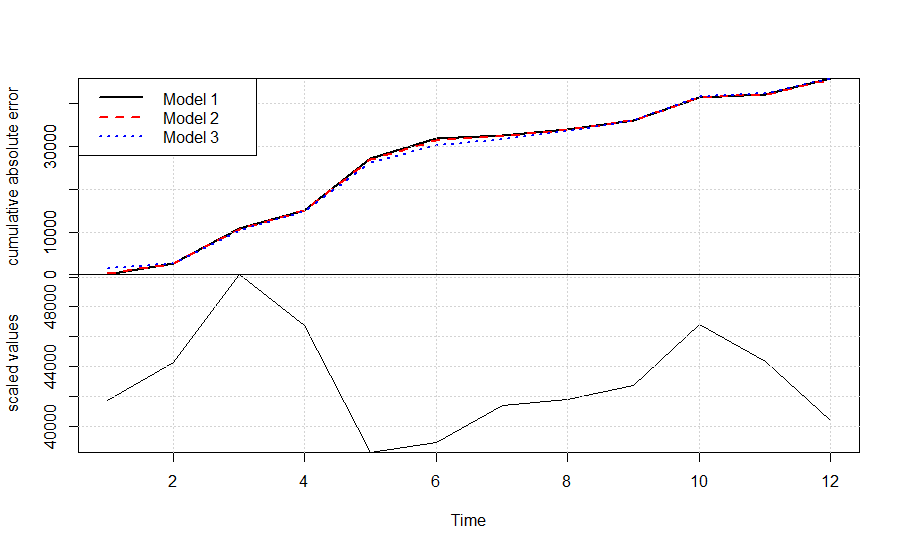
\includegraphics[width=\linewidth]{UK_Model.png}
	\caption{Comparison of the three models fit using the UK data.}
	\label{fig:pairs}
\end{figure}

We can see from the figure above that the predictors added nearly no value in determining GDP per capita. We can also examine the trend, seasonality, and regression components of Model 3 in order to show that the predictors have little-to-no impact on the time series prediction. In this case, let's look at the United States,

\begin{figure}[H]
	\centering
	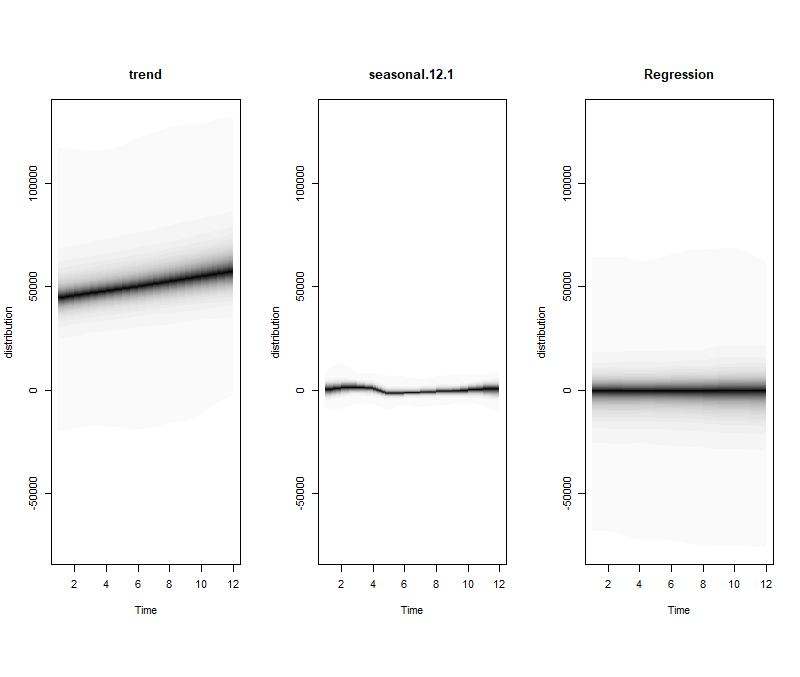
\includegraphics[width=\linewidth]{US_comp.png}
	\caption{Trend, seasonality, and regression components of Model 3 for the US.}
	\label{fig:pairs}
\end{figure}

The bulk of the explanatory power of the model comes from the trend in GDP per capita. The regression predictors add very little to the overall model.

Recall that Model 2 was set to have one explanatory variable. As a result, the model attempted to choose among the three included predictors. We can examine this to help determine the importance of FDI when predicting GDP per capita.

\begin{figure}[H]
	\centering
	\includegraphics[width=\linewidth]{US_Model2_coef.png}
	\caption{Inclusion probabilities for the predictors in Model 2 for the US.}
	\label{fig:pairs}
\end{figure}

As we can see, Foreign Direct Investment has the lowest inclusion probability of the three predictors. This further indicates that the model determined FDI was the last important predictor when forecasting GDP per capita. While only the inclusion probability for the US is shown, this was the case for the models run on all G7 countries. FDI was consistently viewed as the least important predictor by the Bayesian structural time series models.

The only country that saw an improvement in cumulative absolute error after adding the predictors was Italy. We can see a comparison of the three models run on Italy's data below:

\begin{figure}[H]
	\centering
	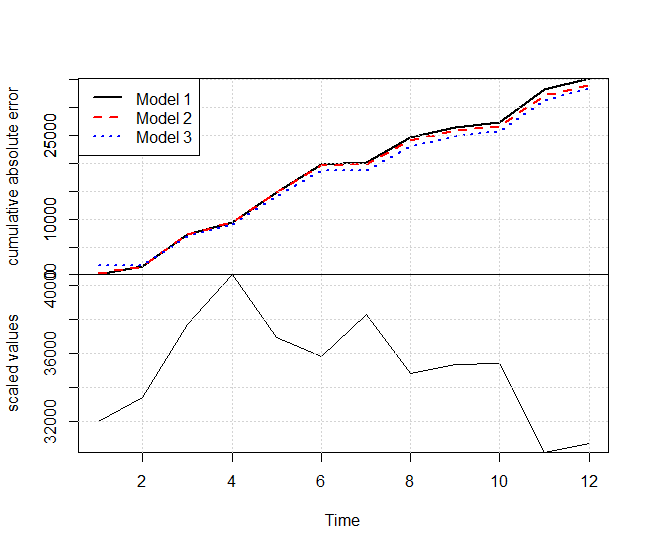
\includegraphics[width=\linewidth]{Italy_Model3.png}
	\caption{Comparison of the three models fit using the Italy data.}
	\label{fig:pairs}
\end{figure}

However, the difference in cumulative absolute error is still quite small. Furthermore, Italy had the lowest GDP per capita and by far the lowest tertiary school completion rate among the G7 countries. The fact that the predictors were more helpful for predicting the GDP per capita of Italy than they were for the other G7 countries lends additional support to the hypothesis that Foreign Direct Investment has a smaller impact on the economies of more advanced countries than it does on their less advanced counterparts.

\newpage
%%%%%%%%%%%%%%%%%%%%%%%%%%%%%%%%%%%%%%
\section{Conclusion}
\quad We can see from the models' outputs that Foreign Domestic Investment is not a significant predictor of GDP per capita growth in high income countries in the 21\textsuperscript{st} century. As a result, the governments of countries with advanced economies may need to more carefully examine trade deals before entering into them. Since Foreign Direct Investment does not confer the same general benefits onto high income countries as it does onto low income countries (improved technology, business practices, etc.), there is a need to thoroughly outline the benefits and drawbacks of increased FDI. It may be the case in some situations in high income countries that domestic investment is preferable to foreign investment.
%%%%%%%%%%%%%%%%%%%%%%%%%%%%%%%%%%%%%%
\section{Future Research}
\quad This paper takes a broad overview of economic data by country in order to determine the ineffectiveness of FDI in increasing GDP per capita among high income countries. As stated in the conclusion, high income countries may need to take a finer look at each situation in order to determine if increased FDI is the correct path to take. A future paper might more closely examine the effect of FDI on specific business situations within an advanced economy. Furthermore, there has been much research on the effects of Foreign Direct Investment on low income countries and this paper focuses on very high income countries \cite{borensztein, hansen}. As a result, there is a gap where middle income countries have been omitted. A future paper may examine the relationship between GDP per capita and FDI among these middle income countries in areas such as Eastern Europe and Latin America.
%%%%%%%%%%%%%%%%%%%%%%%%%%%%%%%%%%%%%%
\newpage
\begin{thebibliography}{9}
\bibitem{borensztein}
Eduardo Borensztein, Jose De Gregorio, Jong-Wha Lee.
\textit{How Does Foreign Direct Investment Affect Economic Growth?}. NBER Working Paper Series, March 1995.

\bibitem{hansen}
Henrik Hansen, John Rand.
\textit{On the Causal Links between FDI and Growth in Developing Countries}.
World Institute for Development Economics Research, June 2005.

\bibitem{scott}
Steven L. Scott. \textit{Fitting Bayesian structural time series with the bsts R package}. The Unofficial Google Data Science Blog, July 2017.
\end{thebibliography}
\end{document}
